%%%%%%%%%%%%%%%%%%%%%%%%%%%%%%%%%%%%%%%%%%%%%%%%%%%%%%%%%%%%%%%%%%%%%%%%%%%%%%%%
%2345678901234567890123456789012345678901234567890123456789012345678901234567890
%        1         2         3         4         5         6         7         8

\documentclass[letterpaper, 10 pt, conference]{ieeeconf}  % Comment this line out if you need a4paper

%\documentclass[a4paper, 10pt, conference]{ieeeconf}      % Use this line for a4 paper

\IEEEoverridecommandlockouts                              % This command is only needed if 
                                                          % you want to use the \thanks command

\overrideIEEEmargins  
% Needed to meet printer requirements.
\usepackage{graphicx}
\usepackage{hyperref}

\usepackage{mathtools}
\usepackage{makecell}
%In case you encounter the following error:
%Error 1010 The PDF file may be corrupt (unable to open PDF file) OR
%Error 1000 An error occurred while parsing a contents stream. Unable to analyze the PDF file.
%This is a known problem with pdfLaTeX conversion filter. The file cannot be opened with acrobat reader
%Please use one of the alternatives below to circumvent this error by uncommenting one or the other
%\pdfobjcompresslevel=0
%\pdfminorversion=4

% See the \addtolength command later in the file to balance the column lengths
% on the last page of the document

% The following packages can be found on http:\\www.ctan.org
%\usepackage{graphics} % for pdf, bitmapped graphics files
%\usepackage{epsfig} % for postscript graphics files
%\usepackage{mathptmx} % assumes new font selection scheme installed
%\usepackage{times} % assumes new font selection scheme installed
%\usepackage{amsmath} % assumes amsmath package installed
\usepackage{amssymb}  % assumes amsmath package installed

\title{\LARGE \bf
Dual-Arm Cooperative Manipulation Through Shared Vision}
\author{Surya Prakash S.K$^{1}$ Ayush Gupta$^{1}$ Suraj S.K$^{2}$ Anudeep D $^{2}$ Karthik T $^{2}$ Sai Teja M$^{2}$ JP Sahoo$^{2}$ \\ Samiran Datta$^{2}$ Amit Shukla$^{2}$ % <-this % stops a space
\thanks{*This work was not supported by any organization.}%
\thanks{$^{1}$S P S. K. is a Research Scholar with the School of Mechanical and Materials Engineering (SMME), Indian Institute of Technology Mandi, H.P., 175005, India (e-mail: {\tt\small s.surya1754@gmail.com}).}%
\thanks{A. Gupta was formerly a Research Scholar with the School of Mechanical and Materials Engineering (SMME), Indian Institute of Technology Mandi, H.P., 175005, India (e-mail: {\tt\small gupta.ayush2587@gmail.com}).}%
\thanks{$^{2}$S. S.K., A .D., K .T., and S T .M. are Research Interns with the Centre for Artificial Intelligence and Robotics (CAIR), Indian Institute of Technology Mandi, H.P., 175005, India (e-mail: {\tt\small surajshaik.in@gmail.com}; {\tt\small anudeep893@gmail.com}; {\tt\small thallamvenkatakarthik@gmail.com}; {\tt\small majjisaiteja12@gmail.com}).}%
\thanks{$^{2}$J. P. Sahoo is a Research Scholar, S. Datta is Research Scholar, and A. Shukla is an Associate Professor with the Centre for Artificial Intelligence and Robotics (CAIR), Indian Institute of Technology Mandi, H.P., 175005, India (e-mail: {\tt\small s23118@students.iitmandi.ac.in}; {\tt\small s24037@students.iitmandi.ac.in}; {\tt\small amitshukla@iitmandi.ac.in}).}}%



\begin{document}

\maketitle
\thispagestyle{empty}
\pagestyle{empty}


%%%%%%%%%%%%%%%%%%%%%%%%%%%%%%%%%%%%%%%%%%%%%%%%%%%%%%%%%%%%%%%%%%%%%%%%%%%%%%%%
\begin{abstract}
This work presents a dual-arm manipulation system using two Kinova Gen3 Lite (6-DOF) manipulators, each equipped with a wrist-mounted eye-in-hand camera, for coordinated target search and pick-and-place in a shared workspace. Each arm independently executes a joint-space search trajectory while performing continuous fiducial (ArUco) marker detection through its own camera. Upon detection by either arm, the target pose is computed in the detecting arm's own base frame via forward kinematics of the eye-in-hand camera and transformed into the other arm's base frame through a calibrated inter-arm reference transform. A reachability-based role-assignment rule then dynamically selects which arm performs the manipulation: the detecting arm, the non-detecting arm, or when the target lies within both arms' reachable workspace, whichever arm is physically closer, independent of which arm made the initial detection. The selected arm executes the pick-and-place sequence using damped least-squares resolved-rate control, with grasp orientation resolved under the gripper's rotational symmetry to minimize unnecessary wrist motion. The complete pipeline: search, detection, cross-frame pose communication, reachability-driven role assignment, and execution is validated in both Gazebo/ROS2 simulation and on physical dual-arm hardware, demonstrating a reproducible, classical-vision-based coordination protocol for dual-arm target acquisition without reliance on learned perception or control components. \textit{Source code and videos for the present work are available at} \href{https://github.com/suryaroboticarm/Shared-Vision-for-Dual-Arm.git}{git-hub} and \href{https://drive.google.com/drive/folders/114Fpy-4yFBnGds0StAoZXTxJKZZoLpme?usp=sharing}{Video}.
\end{abstract}
\begin{keywords}
    Dual-Arm Manipulation, Collaborative Manipulation, Shared Vision, Resolved-Rate Control.
\end{keywords}

%%%%%%%%%%%%%%%%%%%%%%%%%%%%%%%%%%%%%%%%%%%%%%%%%%%%%%%%%%%%%%%%%%%%%%%%%%%%%%%%
\section{INTRODUCTION}
Single-arm manipulators are the standard building block of industrial pick-and-place automation for a fixed, well-characterized workspace, a single arm with a calibrated camera and a repeatable grasp routine is simple to deploy, easy to reason about, and
reliable in operation \cite{shukla2024automated}. This works well as long as every object of interest reliably
falls within that one arm's reachable envelope. As operations scale up, higher throughput cells, larger bins and conveyors, or workspaces shared with other stations this assumption starts to break down: a single arm's reach is fixed, but the region objects can appear in is often larger than what one arm can physically cover. The common industrial response is to bring in a second manipulator to share the same workspace rather than scale up to a single larger (and more expensive) arm, but this immediately introduces a coordination problem \cite{prajapati2025kinematics} that a single-arm system never has to solve: when both arms can potentially act, which one actually should?

Existing work addresses this coordination problem in a few largely distinct ways. One line of work treats both arms as a single coordinated system executing one task jointly synchronized bi-manual grasping, coordinated object handover between the two arms, and cooperative task-space control where both end-effectors track a shared object frame \cite{smith2012dual}. A second line treats coordination as a task allocation and scheduling problem: given a set of discrete objects or sub-tasks, an optimization solver, constraint program, or learned policy decides which robot handles which task, typically using a shared, centrally available state of the workspace (often a single external or overhead camera) \cite{behrens2019constraint, jermann2024efficient}. A third line addresses coordination at the mechanical design stage, using reachability or capability maps computed offline to decide where each arm should be mounted and which regions of the shared workspace belong to which arm, so that task assignment reduces to a static, precomputed zone lookup rather than a runtime decision \cite{zacharias2007capturing}. 

A coordination style that receives comparatively little attention combines two things that are each common on their own, but not typically found together: (i) perception carried independently by each arm itself, via its own wrist-mounted eye-in-hand camera,
rather than a shared external sensor providing a single global view, and (ii) a runtime, per-detection decision of which arm should act, based on live reachability computed in each arm's own frame, rather than a precomputed static zone or a centrally-solved allocation problem. Eye-in-hand vision is well established for single-arm pick-and-place \cite{nguyen2025vision}, and dual-arm eye-in-hand configurations have been used
for tasks such as cooperative 3D scanning \cite{kobayashi2022obtaining}, but in these cases the second arm's camera is not used to help decide which arm should manipulate a shared target. Based on
our review of the literature, dynamic, reachability-based role assignment driven by cross-communicating per-arm eye-in-hand vision rather than a shared external camera or an offline-computed zone assignment is a coordination mode that has not been directly addressed. 

This paper addresses exactly that case. We present a dual-arm system in which two 6-DOF manipulators, each with its own wrist-mounted (eye-in-hand) camera, independently search a shared workspace using a fiducial marker as the target \cite{garrido2014automatic}. Detection by either
arm's camera is followed by a dynamic, reachability-based rule that selects which arm
performs the pick, with the target pose communicated across the arms' base frames
through a calibrated rigid transform regardless of which arm made the detection.
Manipulation itself uses classical resolved-rate control: a damped least-squares
inverse-kinematics formulation for singularity-robust joint velocity control \cite{nakamura1986inverse, chiaverini1994review}, driven by a Cartesian pose error computed directly from live eye-in-hand visual
feedback \cite{hutchinson1996tutorial}. 

We present this deliberately as a small, well-scoped technique rather than a general coordination framework: the contribution is the specific reachability-driven
role-assignment rule and the cross-arm pose communication mechanism that implements it,
validated end-to-end on both a Gazebo/ROS2 simulation and physical Kinova Gen3 Lite hardware. We make no claim beyond this in particular, we do not address continuous visual tracking during manipulation, multi-object scheduling, or bimanual coordinated grasping, each of which is a separate problem in its own right. The contributions of this work are:
\begin{itemize}
\item A runtime reachability-based role-assignment rule that selects the acting arm per detection, resolving workspace overlap by minimum base-to-target distance and resuming the search when neither arm can reach the target.

\item A cross-frame pose relay through a shared calibrated reference transform, which expresses a target detected by one arm's eye-in-hand camera in the other arm's base frame, enabling reachability to be evaluated for both arms without a shared external sensor.

\item End-to-end validation of the full pipeline (concurrent search, cross-frame relay, role assignment, and DLS resolved-rate pick-and-place) in Gazebo/ROS2 and on physical Kinova Gen3 Lite hardware, with source code and videos released publicly.
\end{itemize}
\section{Related Work}
Multi-robot systems are particularly useful when an operation requires an extended workspace or complex, dexterous manipulation. To address these demands, existing literature has proposed diverse coordination frameworks.

In particular, dual-arm manipulators which mirror bi-manual human configurations have gained significant attention for deployment in sorting and object transport applications \cite{surya2025iapf, prajapati2025kinematics}. In collaborative manipulator operations, coordination is achieved in various ways: robots exchange real-time kinematic data \cite{ORTENZI2018110} and goal configurations via wireless communication \cite{10891400}, or they utilize a global motion-capture system for centralized spatial tracking \cite{10843915}.

Early work on dual-arm coordination focused on the case where both arms jointly manipulate a single shared object, requiring their motions and applied forces to be explicitly coupled at the control level. A symmetric hybrid position/force control scheme in which workspace force, velocity, and position vectors are defined as symmetric functions of both arms' joint-space quantities, so that neither arm is treated as dominant over the other \cite{uchiyama1988symmetric}. An alternative and widely
used formulation is the leader-follower (or master/slave) scheme, in which one arm's trajectory is commanded directly and the second arm's motion is derived to accommodate it for example, through generalized master/slave coordination for a dual-arm
system \cite{Caccavale2025}. These approaches, along with related hybrid and adaptive-control variants, are surveyed broadly in \cite{smith2012dual}. In this body of work, coordination is fundamentally about how two arms move together while acting on the same object, rather than about deciding which arm should act. 

A second line of work treats coordination as a discrete assignment problem: given a set of objects, sub-tasks, or motion segments, some mechanism decides which arm is responsible for which. \cite{behrens2019constraint} Formulate simultaneous task allocation and motion scheduling for industrial dual-arm cells as a constraint programming problem, jointly optimizing task order and arm assignment subject to precedence and timing constraints. A related but distinct approach addresses this at the mechanical design stage: \cite{zacharias2007capturing} construct reachability and capability maps that characterize which regions of a workspace a given manipulator can access, which can inform a static division of a shared workspace into per-arm zones computed offline. In both cases, the assignment of a task to an arm is either solved centrally by an optimizer or fixed in advance by workspace geometry, rather than decided at runtime from live sensing at the moment a target is encountered.

More recent work applies learned policies to dual-arm coordination, at both the control and the task-assignment level. \cite{jermann2024efficient} Use reinforcement learning to coordinate multiple robot arms for pick-and-place sorting tasks, learning an assignment and motion policy directly from interaction rather than from a hand-designed allocation rule. \cite{10.3389/frobt.2022.830007} Explore model-free reinforcement learning for dual-arm peg-in-hole assembly, coupling two single-arm controllers through a single centrally learned policy rather than an explicit kinematic or force-level coordination law. Most recently, \cite{11223144} propose a vision-language-model-assisted diffusion framework that predicts object-centric motion flows for each arm from a small number of human demonstrations and dynamically assigns the predicted motions to whichever arm should execute them at a given point in the task. Across this line of work, both the low-level motion and the higher-level question of which arm acts are increasingly folded into a single learned model, in contrast to the explicitly modeled kinematics and hand-specified assignment rules of the present work (Sec.~\ref{kin_model}, Sec.~\ref{reachability}).

The protocol described in this paper sits within this broader landscape as a further, distinct way of achieving cooperation between two arms: it uses classical, explicitly modeled kinematics (Sec.~\ref{kin_model}) throughout, and like the task-allocation approaches above, decides which arm acts based on reachability (Sec.~\ref{reachability}) rather than jointly coupling both arms' motion. It differs from the offline, precomputed workspace division of \cite{zacharias2007capturing} in that reachability is evaluated at runtime for each detected target, using pose information relayed between each arm's own onboard eye-in-hand camera and the other arm's frame, rather than a shared external sensor or a policy learned from interaction. This is presented as one additional point in the existing space of coordination mechanisms, rather than as a replacement for control-level coupling, offline task scheduling, or learned coordination policies, each of which addresses a different aspect of the same underlying multi-arm coordination problem.

\section{Methodology}
\subsection{System Architecture}
The platform consists of two Kinova Gen3 Lite manipulators (6 DOF each),
denoted $\mathcal{A}_L$(LEFT) and $\mathcal{A}_R$(RIGHT), each equipped with a
wrist-mounted (eye-in-hand) RGB camera, sharing a common tabletop workspace. Fig.~\ref{fig:overall} summarizes the complete pipeline described in this section. Both arms first
home concurrently, then search the shared workspace while running marker detection
on their own eye-in-hand camera; once either arm's camera locates the target, the
detected pose is relayed into both arms' own base frames, and a reachability-based
rule selects which arm proceeds to manipulate it, resuming the search if neither arm
can reach it. The selected arm then executes a seven-step pick-and-place sequence, in
which every Cartesian motion stage is driven by the same PD-law-into-damped-least-squares
control loop. Each of these components, the search trajectory, the cross-frame pose
relay, the reachability-based role-assignment rule, the manipulation sequence, and the
underlying resolved-rate control law is described in detail in the subsections below. 
\begin{figure}
    \centering
    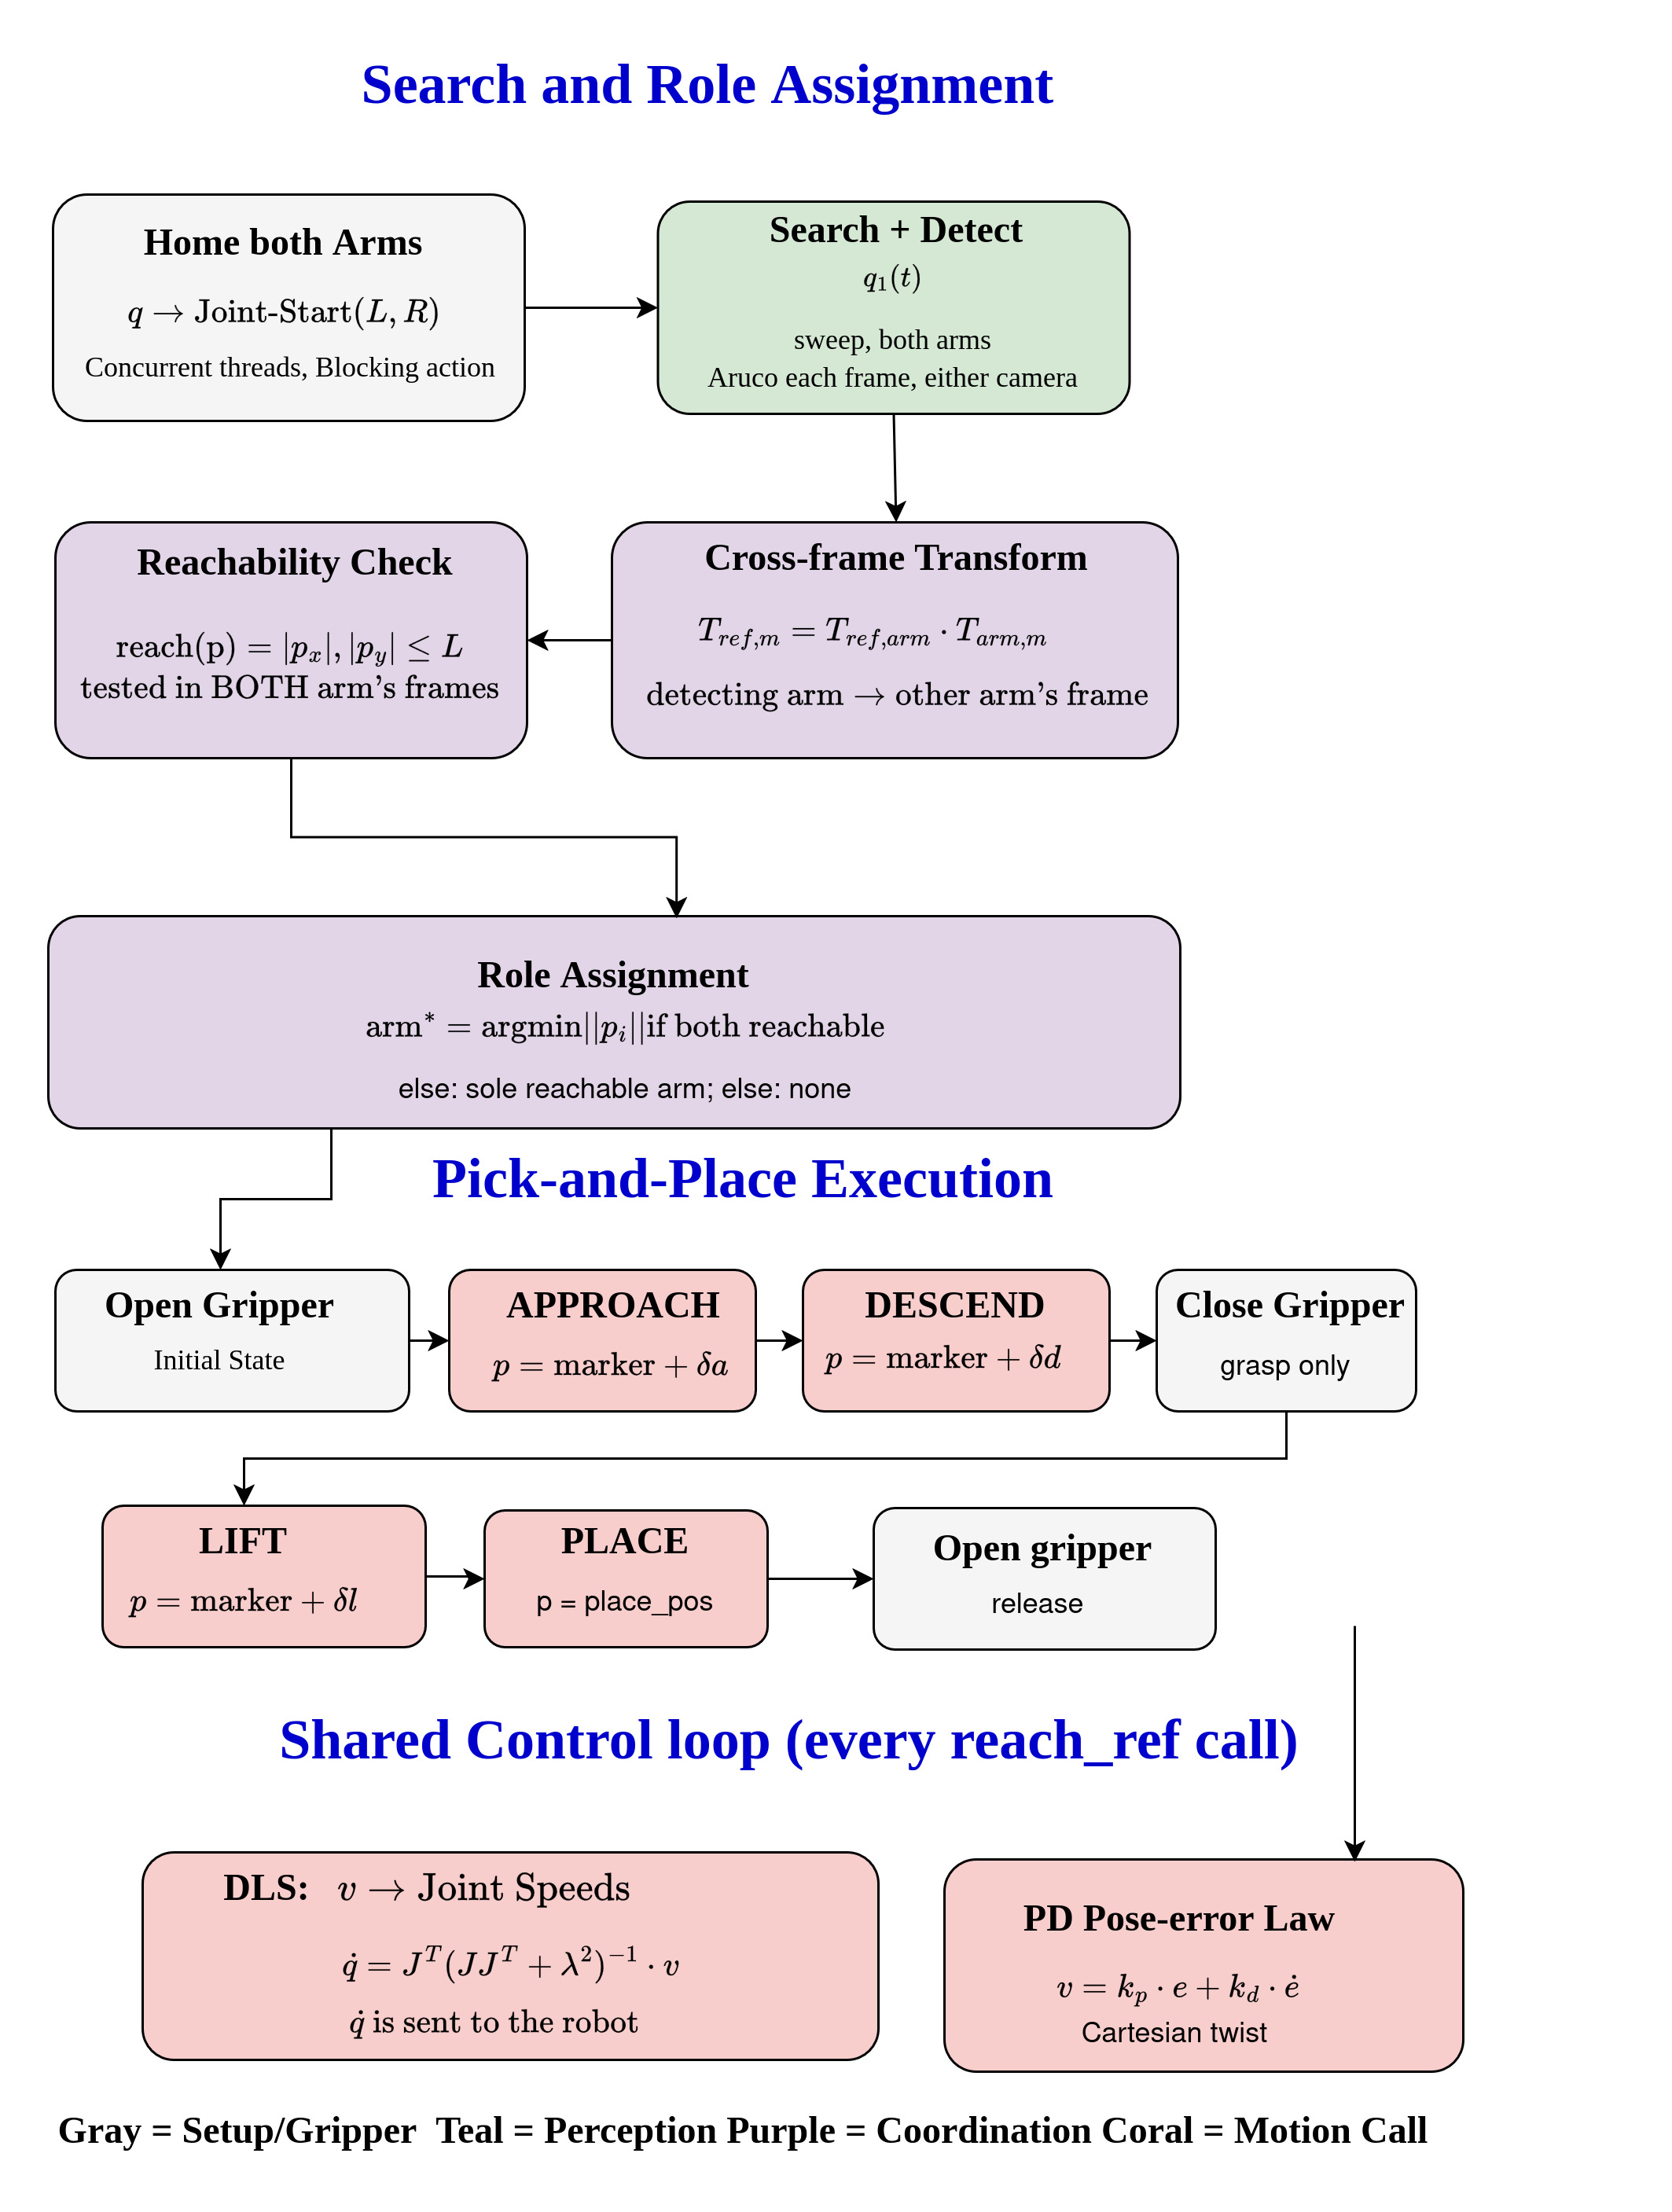
\includegraphics[width=\linewidth]{shared_vision-Shared_vision_overall.jpg}
    \caption{Overall Architecture: concurrent homing and search, cross-frame pose relay, reachability-based role assignment, and pick-and-place execution under the shared PD-into-DLS control loop.}
    \label{fig:overall}
\end{figure}
\subsection{Kinematic Model}
\label{kin_model}
Each arm's forward kinematics is a chain of fixed-geometry, single-DOF homogeneous
transforms Eq.~\ref{fwd_kin}:
\begin{equation}
\begin{aligned}
T_{0}^{6}(\mathbf{q}) &=
T_{0}^{1}(q_{1})
T_{1}^{2}(q_{2})
T_{2}^{3}(q_{3})
T_{3}^{4}(q_{4})
T_{4}^{5}(q_{5})
T_{5}^{6}(q_{6}), \\
\mathbf{q} &= [q_{1}, \cdots, q_{6}] \in \mathbb{R}^{6}.
\end{aligned}
\label{fwd_kin}
\end{equation}
Two further fixed transforms extend the chain to the tool frame and the eye-in-hand
camera frame Eq.~\ref{tool_cam}:
\begin{equation}
\begin{aligned}
T_{0}^{e}(\mathbf{q}) &= T_{0}^{6}(\mathbf{q})\,T_{6}^{e}, \\
T_{0}^{c}(\mathbf{q}) &= T_{0}^{e}(\mathbf{q})\,T_{e}^{c}.
\end{aligned}
\label{tool_cam}
\end{equation}
with $T_6^{e}$ the fixed tool-frame offset and $T_e^{c}$ the fixed eye-in-hand camera offset (identical, by construction, on both arms). The manipulator Jacobian $J(\mathbf q)\in\mathbb R^{6\times 6}$ is obtained by central-difference numerical differentiation of $T_0^{e}$ as in Eq.~\ref{jabob}:
\begin{equation}
\mathbf{J}_{:,i}=
\begin{bmatrix}
\dfrac{\mathbf{p}(\mathbf{q}+\epsilon\mathbf{e}_{i})-
\mathbf{p}(\mathbf{q}-\epsilon\mathbf{e}_{i})}{2\epsilon} \\[1.2ex]
\dfrac{\log\!\left(
\mathbf{R}(\mathbf{q}+\epsilon\mathbf{e}_{i})
\mathbf{R}(\mathbf{q}-\epsilon\mathbf{e}_{i})^{T}
\right)}{2\epsilon}
\end{bmatrix},
\qquad
\epsilon=10^{-6}.
\label{jabob}
\end{equation}
where $\mathbf p(\cdot),R(\cdot)$ are the translational and rotational parts of $T_0^{e}$ and $\mathbf e_i$ is the i-th standard basis vector. The rotation term uses $R^\top$ in place of $R^{-1}$, which is valid because rotation matrices are orthogonal ($R^{-1}=R^\top$ for all $R\in SO(3)$). Unlike position, which lies in a vector space and admits a direct central difference, rotations do not subtract
meaningfully; $\log(\cdot)$ denotes the matrix logarithm mapping a relative rotation $R(\mathbf q+\epsilon\mathbf e_i)R(\mathbf q-\epsilon\mathbf e_i)^\top\in SO(3)$ to its axis-angle vector in $\mathbb R^3$. Since this relative rotation is accumulated over the interval [$-\epsilon,\epsilon$], its rotation vector is approximately $2\epsilon$ times the instantaneous angular velocity direction, so dividing by $2\epsilon$ recovers the angular-velocity Jacobian column exactly as the position rows recover the linear one.

\subsection{Search Trajectory}
\label{search_trajectory}
Both arms first execute a blocking angular Action move (in independent threads, so neither arm idles waiting for the other) to a per-arm predefined start configuration $\mathbf q_0^{L}, \mathbf q_0^{R}$.

Each arm then independently sweeps its own joint 1 at constant angular speed, reversing direction at each bound rather than following a smooth periodic profile as in Eq.~\ref{search_trajec}:
\begin{equation}
\dot{q}_{1}(t)=
\begin{cases}
+\dot{q}_{\mathrm{sweep}}, &
\begin{aligned}[t]
q_{1}(t) &\leq q_{1}^{\max},\\
\mathrm{direction} &= +1,
\end{aligned}
\\[1ex]
-\dot{q}_{\mathrm{sweep}}, &
\begin{aligned}[t]
q_{1}(t) &\geq q_{1}^{\min},\\
\mathrm{direction} &= -1.
\end{aligned}
\end{cases}
\label{search_trajec}
\end{equation}
with direction flipping at each bound, and bounds computed from that arm's own start angle $q_{1,0}$, a sweep half-range $\Delta_{\text{search}}$, and the joint's hard limits $q_1^{\text{lo}}, q_1^{\text{hi}}$ with safety margin $\epsilon$:

\begin{equation}
\begin{aligned}
q_{1}^{\min} &= \max\!\left(q_{1,0}-\Delta_{\mathrm{search}},
\, q_{1}^{\mathrm{lo}}+\epsilon\right), \\
q_{1}^{\max} &= \min\!\left(q_{1,0}+\Delta_{\mathrm{search}},
\, q_{1}^{\mathrm{hi}}-\epsilon\right).
\end{aligned}
\end{equation}
While sweeping, each arm continuously runs ArUco marker detection on its own camera
stream.
\subsection{Visual Target Localization}
Given a detected marker's corner correspondences, a PnP-based pose estimator yields $(\mathbf t_{cm}, R_{cm})$ relative to the camera. Using the live camera pose $T_0^{c}(\mathbf q)$ at the instant of detection, the marker pose is expressed in the detecting arm's own base frame:
\begin{equation}
T^{m}_{arm}
=
T^{c}_{0}(\mathbf{q})\,
T^{m}_c,
\qquad
T^{m}_c
=
\begin{bmatrix}
R_{cm} & \mathbf{t}_{cm} \\
\mathbf{0}^{T} & 1
\end{bmatrix}.
\end{equation}
\subsection{Cross-Frame Pose Communication}
\label{cross_frame}
The two arms' base frames are related by a fixed, calibrated rigid transform $T_{\text{ref}}^{R}\in SE(3)$ (LEFT is the shared reference frame, $T_{\text{ref}}^{L}=I$). The detected marker pose $T_{\text{arm}}^{m}$ is relayed into the shared frame and then into the other arm's own frame by:
\begin{equation}
\begin{aligned}
T^{m}_{\text{ref}}
&= T^{\text{arm}}_{\text{ref}}\,T^{m}_{\text{arm}}, \\
T^{m}_{{\text{arm}}'}
&= \left (T^{\text{arm}'}_{\text{ref}}\right)^{-1}
T^{m}_{\text{ref}}.
\end{aligned}
\end{equation}
This round-trip through the shared frame is what allows a target detected by one
arm's camera to be evaluated in the other arm's own frame, regardless of which arm
made the detection.

\subsection{Reachability-Based Role Assignment}
\label{reachability}
Reachability of a position $\mathbf p$ (expressed in a given arm's own base frame) is tested against that arm's calibrated workspace half-extent $L$:
\begin{equation}
\operatorname{reach}(\mathbf{p})
=
\begin{cases}
1, & |p_x| \leq L_w \text{ and } |p_y| \leq L_w,\\
0, & \text{otherwise}.
\end{cases}
\label{reach_eq}
\end{equation}
Upon detection, $\text{reach}(\cdot)$ is evaluated for both arms using their respective local pose (Sec.~\ref{cross_frame}), and the acting arm is selected as:
\begin{equation}
\mathrm{arm}^{*}=
\begin{cases}
a_d, &
\text{if only } a_d \text{ satisfies } \operatorname{reach},\\[0.5ex]
a_o, &
\text{if only } a_o \text{ satisfies } \operatorname{reach},\\[0.5ex]
\displaystyle
\arg\min_{i\in\{L,R\}}
\|\mathbf{p}_i\|, &
\text{if both satisfy } \operatorname{reach},\\[1ex]
\varnothing, &
\text{otherwise}.
\end{cases}
\end{equation}
where $a_{d}$, $a_{o}$ are detecting and other arm respectively.
% \begin{table}[htbp]
%     \centering
%     \caption{System and controller parameters.}
%     \label{tab:params}
%     \scriptsize
%     \setlength{\tabcolsep}{3pt}
%     \renewcommand{\arraystretch}{1.1}
%     \begin{tabular}{@{}l p{1.45in} r@{}}
%         \hline
%         \textbf{Symbol} & \textbf{Description} & \textbf{Value} \\
%         \hline
%         \multicolumn{3}{@{}l}{\textit{Kinematics and rig geometry}} \\
%         $\epsilon$ & Central-difference step (Eq.~\ref{jabob}) & $10^{-6}$ \\
%         $T^{R}_{\text{ref}}$ & Inter-arm transform (transl.; rot.) & $[1.08,0,0]$~m; $R_z(180^{\circ})$ \\
%         $L_w$ & Workspace half-extent (Eq.~\ref{reach_eq}) & $0.5$~m \\
%         \hline
%         \multicolumn{3}{@{}l}{\textit{Search trajectory}} \\
%         $\dot q_{\mathrm{sweep}}$ & Joint-1 sweep speed & $8^{\circ}$/s \\
%         $\Delta_{\mathrm{search}}$ & Sweep half-range & $120^{\circ}$ \\
%         $\delta_{\mathrm{lim}}$ & Joint-limit safety margin & $0.08$~rad \\
%         \hline
%         \multicolumn{3}{@{}l}{\textit{Perception}} \\
%         - & ArUco dictionary & \texttt{5X5\_50} \\
%         - & Marker side length & $0.05$~m \\
%         \hline
%         \multicolumn{3}{@{}l}{\textit{Manipulation waypoints}} \\
%         $\mathbf a$ & Approach offset, $\mathcal{A}_L$ / $\mathcal{A}_R$ & $[.05,.02,.07]$ / $[.03,.07,.07]$~m \\
%         $d$ & Descend distance & $0.08$~m \\
%         $l$ & Lift height & $0.10$~m \\
%         \hline
%         \multicolumn{3}{@{}l}{\textit{Resolved-rate control}} \\
%         $K_{p}^{\mathrm{pos}}$, $K_{d}^{\mathrm{pos}}$ & Position PD gains & $2.0$, $0.05$ \\
%         $K_{p}^{\mathrm{ori}}$, $K_{d}^{\mathrm{ori}}$ & Orientation PD gains & $0.9$, $0.04$ \\
%         $\tau$ & Derivative filter time constant & $0.06$~s \\
%         $\lambda$ & DLS damping (nominal / singular) & $0.12$ / $0.45$ \\
%         $w_{\min}$ & Manipulability switch threshold & $0.01$ \\
%         $\dot q_{\max}$ & Joint-speed saturation & $0.2$~rad/s \\
%         - & Control loop rate & $10$~Hz \\
%         \hline
%         \multicolumn{3}{@{}l}{\textit{Convergence tolerances}} \\
%          - & Pos./ori., APPROACH, LIFT, PLACE & $8$~mm / $5^{\circ}$ \\
%          - & Pos./ori., DESCEND (grasp) & $5$~mm / $3^{\circ}$ \\
%          - & Consecutive cycles in tolerance & $3$ \\
%         \hline
%     \end{tabular}
% \end{table}
\begin{table}[htbp]
    \centering
    \caption{System and controller parameters.}
    \label{tab:params}
    \scriptsize
    \setlength{\tabcolsep}{3pt}
    \renewcommand{\arraystretch}{1.1}
    \begin{tabular}{@{}l p{1.45in} r@{}}
        \hline
        \textbf{Symbol} & \textbf{Description} & \textbf{Value} \\
        \hline
        \multicolumn{3}{@{}l}{\textit{Kinematics and rig geometry}} \\
        $\epsilon$ & Central-difference step & $10^{-6}$ \\
        $T^{R}_{\text{ref}}$ & Inter-arm transform (transl.; rot.) & $[1.08,0,0]$~m; $R_z(180^{\circ})$ \\
        $L_w$ & Workspace half-extent & $0.5$~m \\
        \hline
        \multicolumn{3}{@{}l}{\textit{Search trajectory}} \\
        $\dot q_{\mathrm{sweep}}$ & Joint-1 sweep speed & $8^{\circ}$/s \\
        $\Delta_{\mathrm{search}}$ & Sweep half-range & $120^{\circ}$ \\
        $\delta_{\mathrm{lim}}$ & Joint-limit safety margin & $0.08$~rad \\
        \hline
        \multicolumn{3}{@{}l}{\textit{Perception}} \\
        - & ArUco dictionary & \texttt{5X5\_50} \\
        - & Marker side length & $0.05$~m \\
        \hline
        \multicolumn{3}{@{}l}{\textit{Manipulation waypoints}} \\
        $\mathbf a$ & Approach offset, $\mathcal{A}_L$ / $\mathcal{A}_R$ & $[.05,.02,.07]$ / $[.03,.07,.07]$~m \\
        $d$ & Descend distance & $0.08$~m \\
        $l$ & Lift height & $0.10$~m \\
        \hline
        \multicolumn{3}{@{}l}{\textit{Resolved-rate control}} \\
        $K_{p}^{\mathrm{pos}}$, $K_{d}^{\mathrm{pos}}$ & Position PD gains & $2.0$, $0.05$ \\
        $K_{p}^{\mathrm{ori}}$, $K_{d}^{\mathrm{ori}}$ & Orientation PD gains & $0.9$, $0.04$ \\
        $\tau$ & Derivative filter time constant & $0.06$~s \\
        $\lambda$ & DLS damping (nominal / singular) & $0.12$ / $0.45$ \\
        $w_{\min}$ & Manipulability switch threshold & $0.01$ \\
        $\dot q_{\max}$ & Joint-speed saturation & $0.2$~rad/s \\
        - & Control loop rate & $10$~Hz \\
        \hline
        \multicolumn{3}{@{}l}{\textit{Convergence tolerances}} \\
         - & Pos./ori., APPROACH, LIFT, PLACE & $8$~mm / $5^{\circ}$ \\
         - & Pos./ori., DESCEND (grasp) & $5$~mm / $3^{\circ}$ \\
         - & Consecutive cycles in tolerance & $3$ \\
        \hline
    \end{tabular}
\end{table}
\subsection{Manipulation Sequence}
Once $\text{arm}^\star$ is selected, it executes: open gripper; APPROACH; DESCEND; close gripper (grasp); LIFT; PLACE; open gripper (release). Only APPROACH, DESCEND, and LIFT are derived from the marker position $\mathbf p_m$ (in $\text{arm}^\star$'s
own frame); each is built from the previous target rather than independently offset from the marker, and grasp itself involves no motion target:
\begin{equation}
\begin{aligned}
\mathbf{p}_{\mathrm{approach}}
&=
\mathbf{p}_{m}+\mathbf{a}, \\
\mathbf{p}_{\mathrm{descend}}
&=
\mathbf{p}_{\mathrm{approach}}
-
\begin{bmatrix}
0\\
0\\
d
\end{bmatrix}, \\
\mathbf{p}_{\mathrm{lift}}
&=
\mathbf{p}_{\mathrm{descend}}
+
\begin{bmatrix}
0\\
0\\
l
\end{bmatrix}.
\end{aligned}
\end{equation}

where $\mathbf a$ is a fixed per-arm approach offset and $d,l$ are fixed scalar
descend/lift distances (grasp is a gripper actuation at $\mathbf p_{\text{descend}}$,
not a fifth target). The PLACE target $\mathbf p_{\text{place}}$ is, by contrast, a
fixed pre-configured drop-off pose for $\text{arm}^\star$, independent of
$\mathbf p_m$. Grasp yaw is resolved under the gripper's $180^{\circ}$ symmetry by choosing, of the two equivalent orientations, whichever has greater quaternion alignment with the arm's current tool orientation, minimizing unnecessary wrist rotation.
\subsection{Resolved-Rate Motion Control}
Every one of the four motion targets above (APPROACH, DESCEND, LIFT, PLACE) is
reached by the same control loop. Given position/orientation error
$(\mathbf e_p, \mathbf e_o, \theta_e)$ between the current and target tool pose, a PD
law with a first-order low-pass filtered derivative produces a Cartesian twist $\mathbf v$ an intermediate quantity, not a robot command:
\begin{equation}
\mathbf{v}
=
\begin{bmatrix}
K_{p}^{\mathrm{pos}}\,\mathbf{e}_{p}
+
K_{d}^{\mathrm{pos}}\,\dot{\mathbf{e}}_{p,\mathrm{filt}}
\\[1ex]
K_{p}^{\mathrm{ori}}\,\mathbf{e}_{o}
+
K_{d}^{\mathrm{ori}}\,\dot{\mathbf{e}}_{o,\mathrm{filt}}
\end{bmatrix}.
\end{equation}
This is mapped to the joint speeds actually sent to the arm via damped least-squares
(DLS) inverse differential kinematics:
\begin{equation}
\dot{\mathbf{q}}
=
J^{T}
\left(
JJ^{T}
+
\lambda^{2}I
\right)^{-1}
\mathbf{v}.
\end{equation}
with $\lambda$ switched between a nominal and a larger value near singularities using the manipulability measure $w(\mathbf q)=\sqrt{\det(JJ^\top)}$ and $\dot{\mathbf q}$ scaled near joint limits and saturated at $\dot q_{\max}$ before being sent.

Position error is a plain vector difference between the target and current tool position:
\begin{equation}
\mathbf{e}_{p}
=
\mathbf{p}^{\star}
-
\mathbf{p}(\mathbf{q}).
\label{position_e}
\end{equation}
Orientation error requires more care, since two rotations cannot simply be subtracted. First, the relative error quaternion between the target and current tool orientation is computed, then sign-corrected so the controller always takes the shorter rotational path:
\begin{equation}
\begin{aligned}
\mathbf{q}_{e}
&=
\mathbf{q}_{\mathrm{tgt}}
\otimes
\mathbf{q}_{\mathrm{curr}}^{-1}, \\
\mathbf{q}_{e}
&\leftarrow
-\mathbf{q}_{e},
\qquad
\text{if } q_{e}^{(4)} < 0.
\end{aligned}
\end{equation}
where $\mathbf q_{\text{tgt}}$  and $\mathbf q_{\text{curr}}$ are the target and current tool orientations as unit quaternions, $\otimes$ is quaternion multiplication, and $q_e^{(4)}$ is the scalar (w) component of $\mathbf q_e$ the sign flip exploits the
fact that a quaternion and its negation represent the same rotation, so it removes the ambiguity that would otherwise let the controller occasionally rotate the long way around.

Writing $\mathbf q_e^{(1:3)}$ for the vector(x, y, z) part of $\mathbf q_e$, the orientation error vector actually used by the PD law is:
\begin{equation}
\mathbf{e}_{o}
=
2\,\mathbf{q}_{e}^{(1:3)}.
\label{qe}
\end{equation}
and the total rotation angle still remaining used only to test convergence, not fed into the control law is recovered exactly (rather than approximated) via:
\begin{equation}
\theta_{e}
=
2\,\operatorname{atan2}\!\left(
\left\|
\mathbf{q}_{e}^{(1:3)}
\right\|,
q_{e}^{(4)}
\right).
\label{arceq}
\end{equation}

Eq.~\ref{qe} follows from the quaternion-to-axis-angle relation
$\mathbf q_e = \big(\sin(\theta_e/2)\,\hat{\mathbf n},\ \cos(\theta_e/2)\big)$, where $\hat{\mathbf n}$ is the rotation axis: the vector part is $\sin(\theta_e/2)\hat{\mathbf n}$, so doubling it gives $2\sin(\theta_e/2)\hat{\mathbf n} \approx \theta_e\hat{\mathbf n}$ for small errors the familiar axis-scaled-by-angle error vector. atan2 is used in Eq.~\ref{arceq}, for numerical stability across the full range of $\theta_{e}$, including near $0^{\circ}$ and $180^{\circ}$.

Convergence is declared once $\lVert\mathbf e_p\rVert$ (Eq.~\ref{position_e}) and $\theta_e$ (Eq.~\ref{arceq})
remain within tolerance for three consecutive control cycles, after which the next waypoint's target is computed and the loop repeats.
\begin{figure}
    \centering
    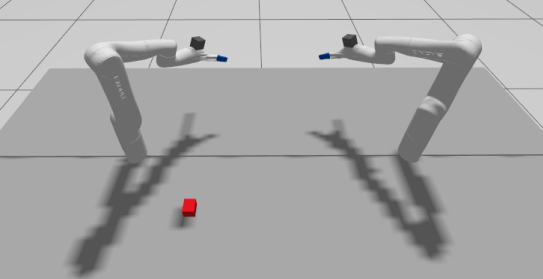
\includegraphics[width=\linewidth]{sim_setup.png}
    \caption{Gazebo/ROS2 simulation setup: two Kinova Gen3 Lite arms sharing a tabletop workspace with a fiducial target.}
    \label{fig:sim_setup}
\end{figure}
\begin{figure}
    \centering
    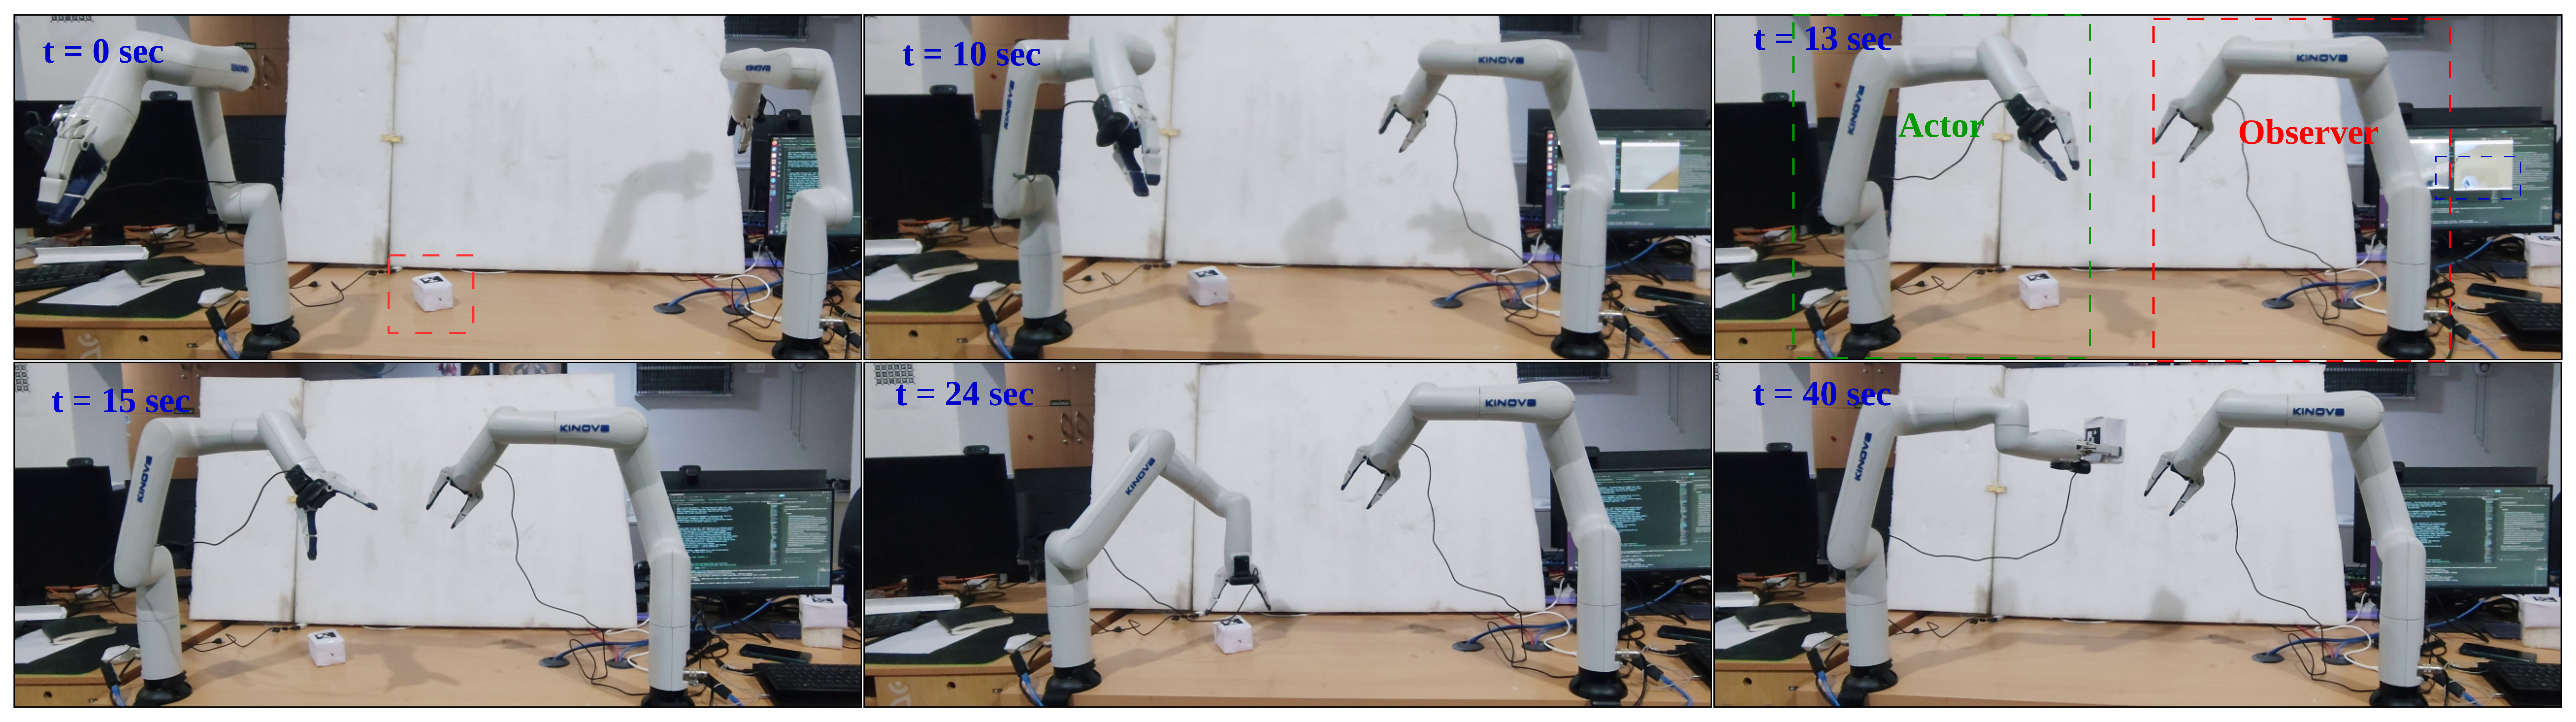
\includegraphics[width=\linewidth]{shared_vision-Page-3(1).jpg}
    \caption{Experiment 1 (hardware): LEFT arm selected as actor, RIGHT arm idle. Frames show search, detection, approach, grasp, and place.}
    \label{fig:exp-1}
\end{figure}
The complete pipeline: homing, concurrent search, cross-frame pose communication,
reachability-based role assignment, and the full manipulation sequence, has been
validated in both Gazebo/ROS simulation as shown in Fig.~\ref{fig:sim_setup} and on physical Kinova Gen3 Lite dual-arm
hardware as shown in Fig.~\ref{fig:exp-1}.
\section{Results and Discussion}
\begin{figure}
    \centering
    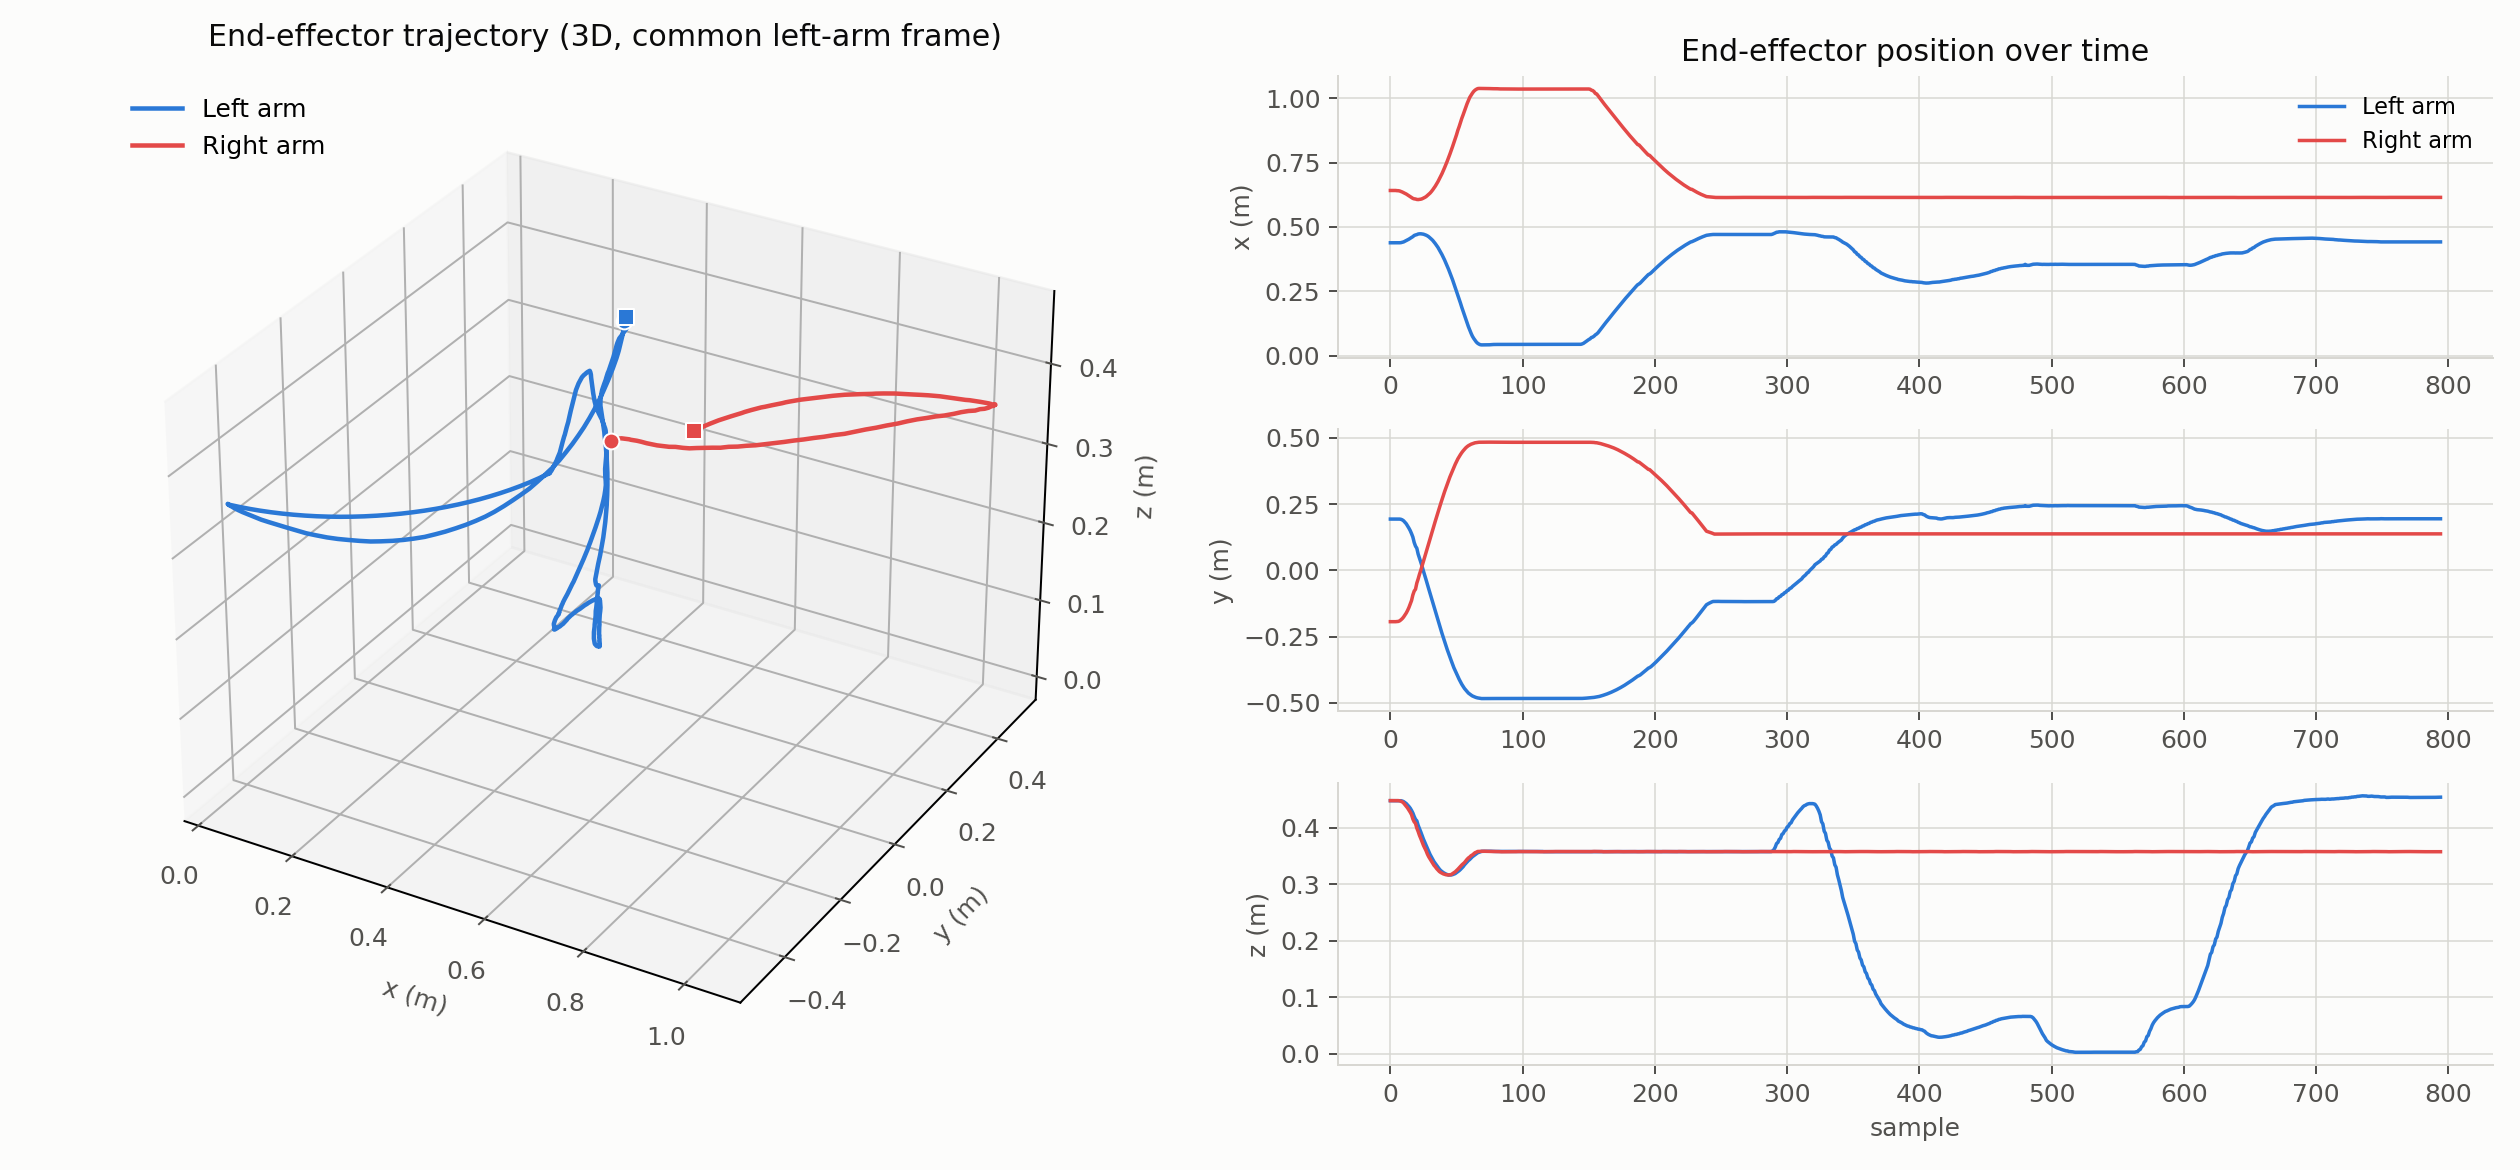
\includegraphics[width=1\linewidth]{end_effector_trajectories_left.png}
    \caption{Experiment 1: end-effector trajectories in the common LEFT-arm frame (left) and per-axis position over time (right). LEFT traces approach–descend–lift–place; RIGHT remains stationary.}
    \label{fig:left_arm}
\end{figure}
\begin{figure}
    \centering
    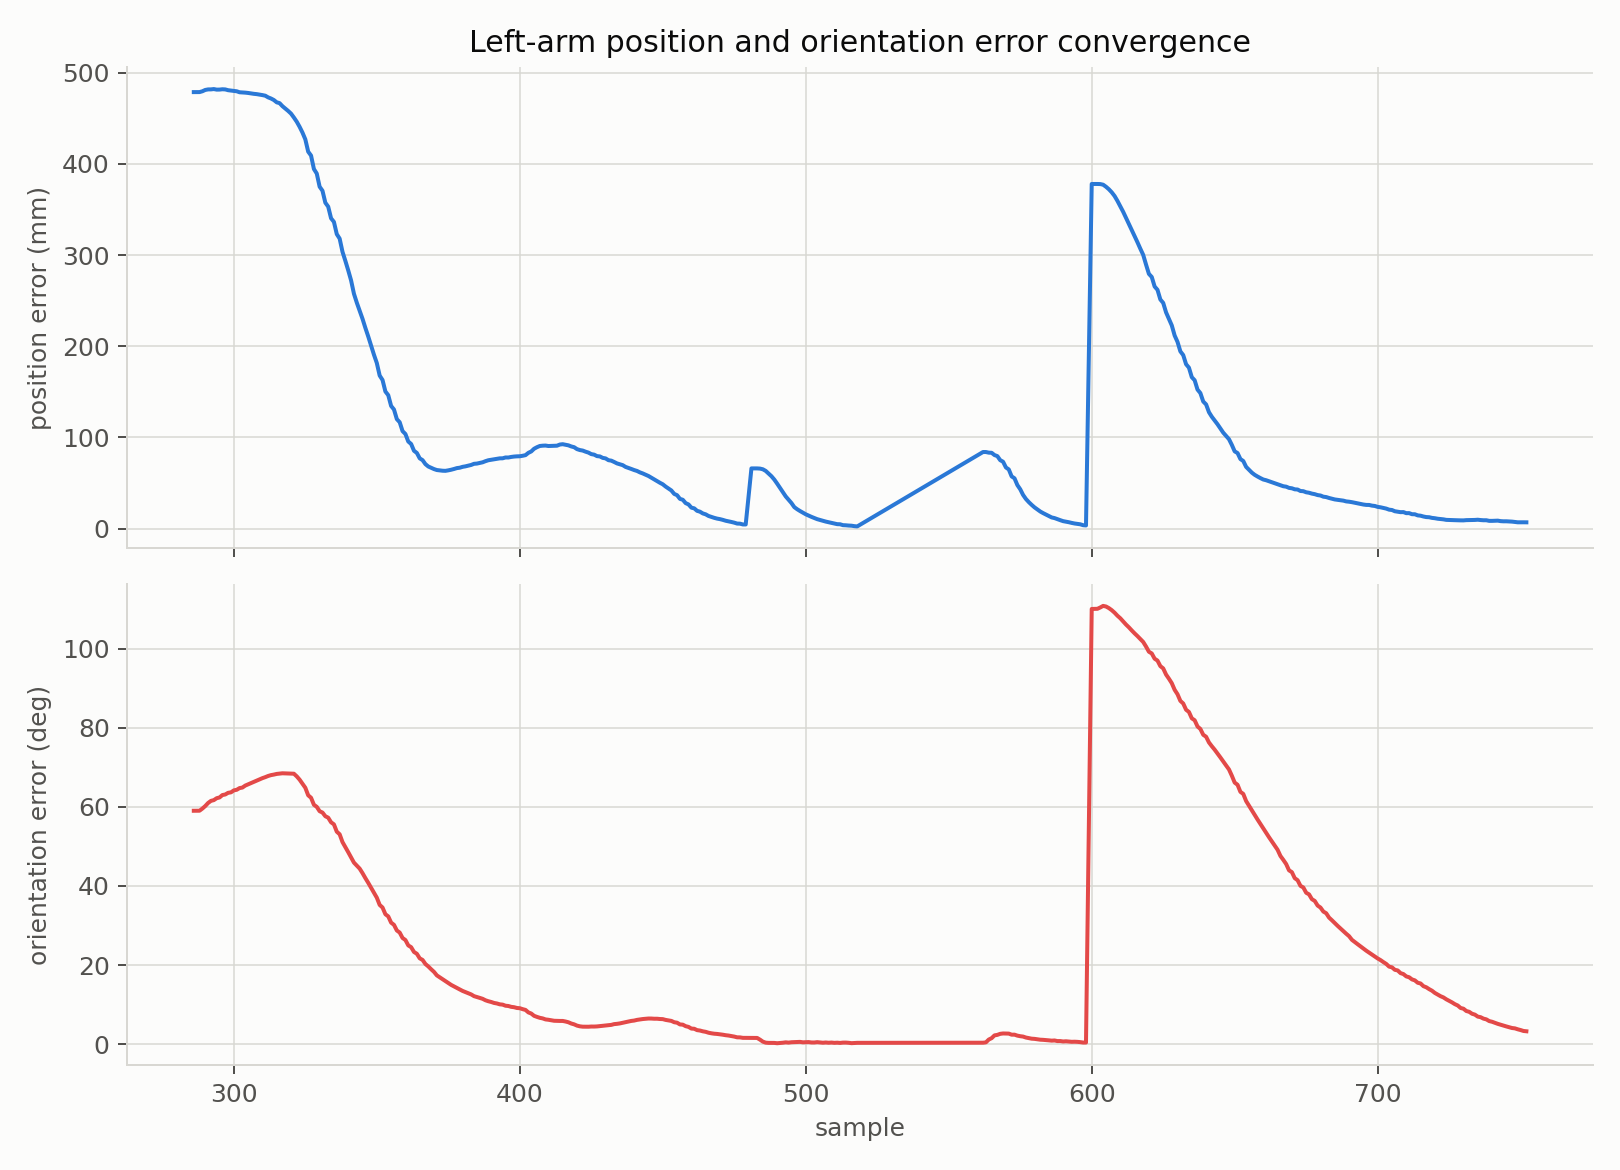
\includegraphics[width=0.7\linewidth]{error_convergence_left.png}
    \caption{Experiment 1: LEFT-arm position and orientation error, showing a convergence transient at each waypoint transition.}
    \label{fig:left_arm_error}
\end{figure}

\begin{figure}
    \centering
    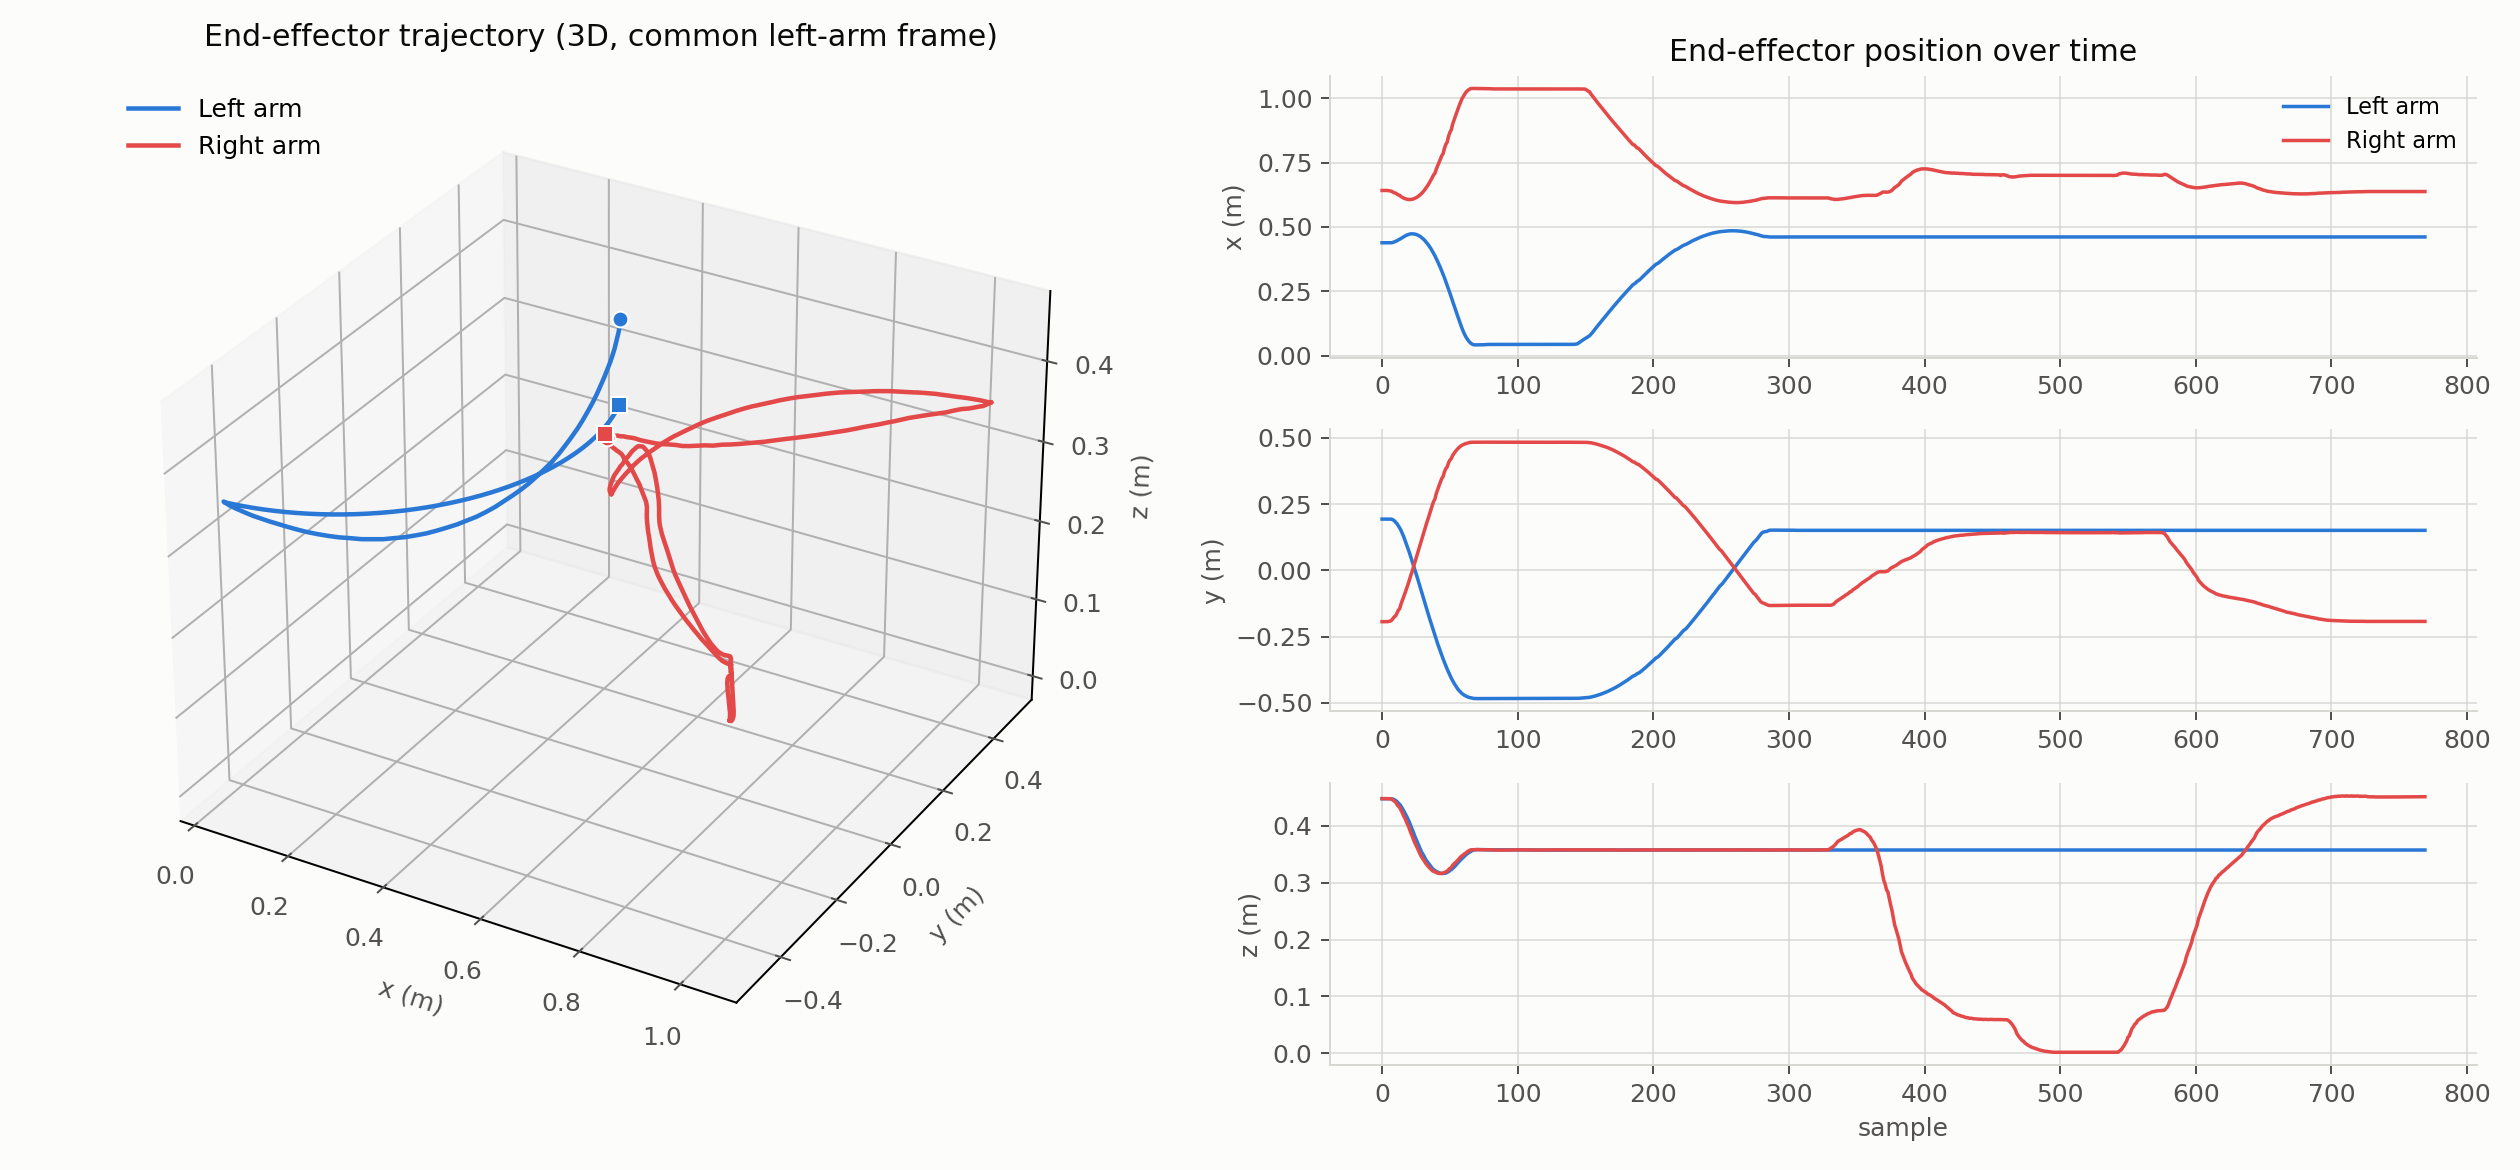
\includegraphics[width=1\linewidth]{end_effector_trajectories_right.png}
    \caption{Experiment 2: end-effector trajectories and per-axis position with RIGHT selected as actor and LEFT idle the mirrored case of Fig.~\ref{fig:left_arm}.}
    \label{fig:right_arm}
\end{figure}
\begin{figure}
    \centering
    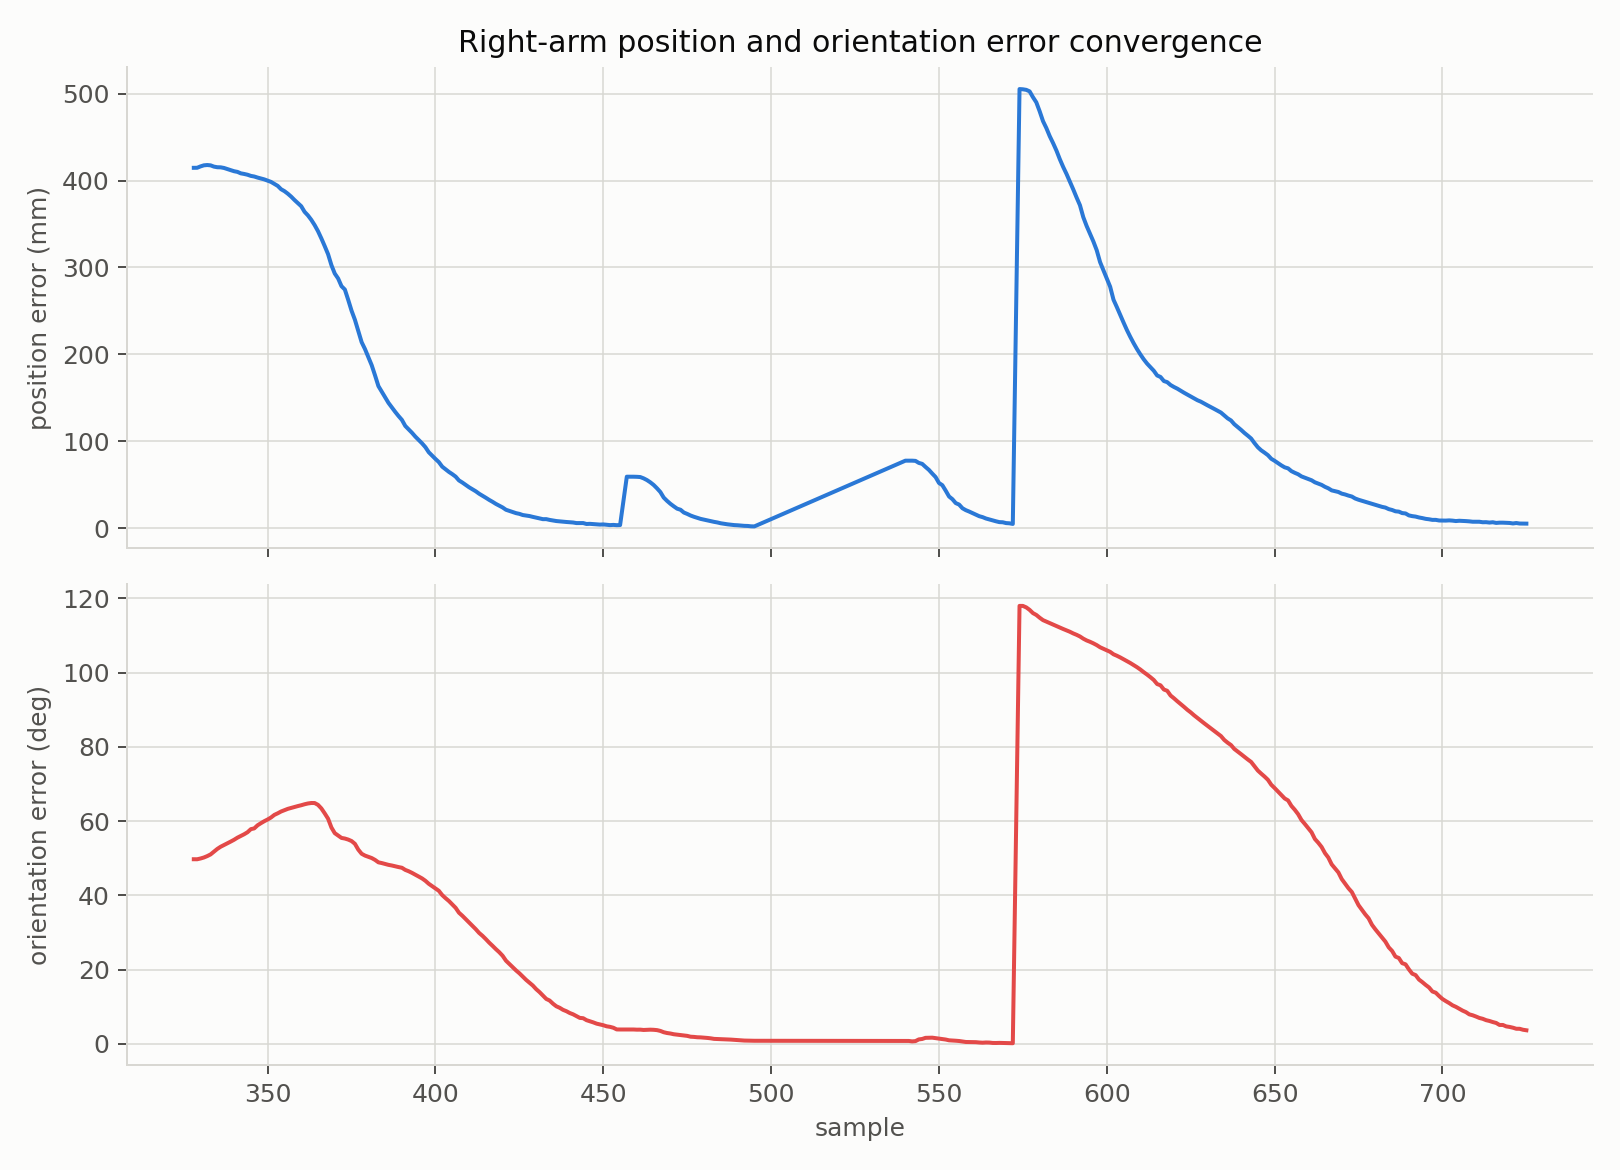
\includegraphics[width=0.7\linewidth]{error_convergence_right.png}
    \caption{Experiment 2: RIGHT-arm position and orientation error convergence.}
    \label{fig:right_arm_error}
\end{figure}


\begin{table}[htpb]
    \centering
    \renewcommand{\arraystretch}{1.4}
    \caption{Final position and orientation error at declared convergence, over five trials with each arm selected as actor.}
    \begin{tabular}{ccc}
        \hline
        \multicolumn{3}{c}{\textbf{Left}} \\
        \hline
        \textbf{Trials} & \textbf{Pos\_error (mm)} & \textbf{Orn\_error (deg)} \\
        \hline
        1 & 2.549 & 0.310 \\
        2 & 2.553 & 0.780 \\
        3 & 4.587 & 0.053 \\
        4 & 3.257 & 1.222 \\
        5 & 2.818 & 0.715 \\
        \hline
        \textbf{Mean} & \textbf{3.153} & \textbf{0.616} \\
        \textbf{Std. Dev.} & \textbf{0.852} & \textbf{0.451} \\
        \hline
        \multicolumn{3}{c}{\textbf{Right}} \\
        \hline
        \textbf{Trials} & \textbf{Pos\_error (mm)} & \textbf{Orn\_error (deg)} \\
        \hline
        1 & 2.183 & 0.842 \\
        2 & 2.640 & 0.767 \\
        3 & 3.144 & 0.641 \\
        4 & 2.447 & 1.023 \\
        5 & 3.397 & 0.156 \\
        \hline
        \textbf{Mean} & \textbf{2.762} & \textbf{0.686} \\
        \textbf{Std. Dev.} & \textbf{0.500} & \textbf{0.327} \\
        \hline
    \end{tabular}
    \label{error_metrics}
\end{table}
Two representative hardware trials illustrate the complete pipeline end-to-end: in Experiment 1, the LEFT arm was selected as the acting arm (Fig.~\ref{fig:exp-1}, Fig.~\ref{fig:left_arm}, Fig.~\ref{fig:left_arm_error}), while in Experiment 2 the RIGHT arm was selected (Fig.~\ref{fig:right_arm}, Fig.~\ref{fig:right_arm_error}), with the non-selected arm remaining idle in each case.

Fig.~\ref{fig:left_arm} shows the LEFT arm's end-effector tracing the full waypoint sequence approach,
descend, lift, and place, while the RIGHT arm's position remains essentially flat across the same sample range, consistent with it never receiving a motion command once the reachability-based rule assigned the task to LEFT. The corresponding error convergence in Fig.~\ref{fig:left_arm_error} shows the position and orientation error dropping from its initial value toward zero, then rising again before converging a second time later in the sequence, reflecting that each waypoint transition presents the resolved-rate controller with a fresh, non-zero error that must be driven back down under the same PD-into-DLS loop, rather than the arm tracking a single continuous trajectory.

Fig.~\ref{fig:right_arm} and Fig.~\ref{fig:right_arm_error} show the mirrored case, with RIGHT selected as the acting arm and
LEFT idle. The same qualitative pattern holds a stationary idle arm and successive convergence transients on the acting arm, indicating that the pipeline behaves consistently regardless of which arm the reachability rule selects, rather than one arm's kinematics or camera calibration producing systematically different convergence behavior than the other's.

Table~\ref{error_metrics} reports the position and orientation error at the point convergence was declared, across five trials with \textbf{Left} selected as the acting arm and five trials with \textbf{Right} selected. Mean final position error was 3.153~mm (\textbf{Left}) and 2.762~mm (\textbf{Right}), with orientation error of 0.616$^\circ$ (\textbf{Left}) and 0.686$^\circ$ (\textbf{Right}); standard deviations were under 1~mm and under 0.5$^\circ$ in both cases. These figures indicate that the resolved-rate control loop consistently reaches sub-5~mm, sub-1.3$^\circ$ final accuracy independent of which arm is assigned the task, suggesting no meaningful asymmetry between the two arms' manipulation precision despite their different mounting positions and per-arm approach offsets. Consistent with the minimal-demo scope of this validation, these five trials per arm establish repeatability at a proof-of-concept level rather than constituting a fully powered statistical characterization of the system.
\section{Conclusion}
This paper presented a dual-arm manipulation system in which two Kinova Gen3 Lite manipulators, each equipped with its own wrist-mounted eye-in-hand camera, independently search a shared workspace and cooperate through a reachability-based role-assignment rule: whichever arm can actually reach a detected target performs the pick, with the target's pose relayed between the two arms' base frames regardless of which arm made
the detection. The complete pipeline concurrent search, cross-frame pose communication, reachability-based selection, and a damped least-squares resolved-rate manipulation sequence was implemented and validated end-to-end in both Gazebo/ROS2
simulation and on physical dual-arm hardware. Across five trials with each arm acting as the selected arm, the system consistently converged to sub-5~mm position error and sub-1.3$^\circ$ orientation error, with no meaningful difference in precision between the two arms, indicating that the coordination protocol performs consistently regardless of which arm is assigned the task. 

This validation should be read within its intended scope. The experiments reported here are a small number of trials per configuration, sufficient to establish repeatability at a proof-of-concept level but not a fully powered statistical characterization; the reachability test itself is a simple axis-aligned workspace box rather than a full manipulability or collision-aware reachability model; and the arm-selection tie-break under workspace overlap uses plain Euclidean distance rather than any measure of manipulability or motion cost. Role assignment is also decided once, at the moment of detection, the system does not currently monitor whether the acting arm's own view of the target remains usable once manipulation begins.

That last point is the most direct avenue for future work: extending the present protocol so that the idle arm continues observing the target during the acting arm's approach, and relays a corrected pose if the acting arm's own eye-in-hand view degrades
mid-task, would move the coordination decision from a one-time handoff to a continuously monitored one. Beyond this, natural extensions include testing the protocol against a larger and more varied set of trials to characterize failure modes more rigorously, replacing the fixed workspace-box reachability test with a learned or manipulability-weighted reachability measure, and extending the single-object handling demonstrated here to multi-object scheduling across the two arms.
\bibliographystyle{ieeetr}
\bibliography{ref}



\end{document}
